\chapter{Summary of Progress}

\section{Data Preparation}

All of the datasets necessary for the analysis has been gathered. Most of
it has been downloaded from public sources on the Internet, using Shell and R
scripts. The wind dataset has been provided by Yesubabu Viswanadhapalli, and
is the result of the assimilation of QuickScat satellite and all available
in situ data in the Red Sea into
the Weather Research and Forecasting (WRF) regional Red Sea model. There are
additional datasets that will be useful for the analysis, but they are mainly
climate mode time-series like IMI and EAWR, that are easy to download. The
downloaded data is listed and described in table \ref{tab:data}.

So far, the MODIS and CCI data have been cropped over the region of interest,
cleaned and exported to the format TIFF, which can be easily read by most
software, R in particular. Each dataset has then been aggregated in a single
file in the native R raster format. Applying this processing to the remaining
raster data should be straightforward. Then, the data will need to be aligned
and aggregated on the same temporal and spatial resolution, before aggregating
it in table format.

\afterpage{

\thispagestyle{empty}

\begin{landscape}
\begin{table}
\centering 
\begin{tabular}{l c c ccc c} 

\toprule 
Variable & Description             & Mission/Source    & Unit                 & Temporal   & Period & Spatial    \\
         &                         &                   &                      & Resolution &        & Resolution \\
\midrule 

CHL      & Chlorophyll             & CCI               & mg/m${}^3$           & 8-days     & 1997-2012 & 4km   \\
SST      & Sea Surface Temperature & MODIS             & Celsius              & 8-days     & 2002-2015 & 4km   \\
AOD      & Aerosol Optical Depth   & MODIS             & N/A                  & daily      & 2000-2015 & 28km  \\
CDOM     & Colored Dissolved       & MODIS             & N/A                  & 8-days     & 2002-2015 & 4km   \\
         & Organic Matter          &                   &                      &            &           &       \\
NAO      & North Atlantic          & NOAA              & N/A                  & daily      & 1979-2015 &  N/A  \\
         & Oscillation Index       &                   &                      &            &           &       \\
PAR      & Photosynthetically      & MODIS             & Einstein/m${}^2$.Day & 8-days     & 2002-2015 &  4km  \\
         & Available Radiations    &                   &                      &            &           &       \\
POC      & Particulate Organic     & MODIS             & mg/m${}^3$           & 8-days     & 2002-2015 &  4km  \\
         & Carbon                  &                   &                      &            &           &       \\
RAIN     & Precipitations          & TRMM              & mm/h                 & daily      & 1998-2015 & 28km  \\
SOI      & Southern Oscillation    & Australian Bureau & N/A                  & daily      & 1999-2015 &  N/A  \\
         & Index                   & of Meteorology    &                      &            &           &       \\
SLA      & Sea Level Anomaly       & Aviso             & cm                   & daily      & 1993-2013 &  28km \\
WIND     & Vector Wind Field       & Simulated         & m/s                  & 3-hourly   & 2000-2014 &  10km \\

\bottomrule

\end{tabular}
\caption{Downloaded data}
\label{tab:data}
\end{table}
\end{landscape}

\clearpage% Flush page
}



\section{Red Sea Chlorophyll Data Analysis}

The MODIS and CCI chlorophyll data products have been explored and compared.
The MODIS data include an important amount of missing data, which may reach
100\% during summer in the southern Red Sea, increasing the complexity of any
analysis in this region. The CCI data product solves this issue by merging
three sources of remotely-sensed chlorophyll data (MODIS, MERIS and SeaWiFS)
and using a new algorithm for retrieving chlorophyll values when the cloud
cover is important.  This increases the coverage to 70\% during summer months
in the southern Red Sea.

The SeaWiFS chlorophyll data has been used in the submitted companion article
of Chapter 3 (see Appendice B).  The seasonal signal in the data is strong and
has been shown to account for 50\% of the variability. The seasonal anomalies
display a strong spatio-temporal correlation: the temporal correlation of
anomalies is 40\%, whereas two locations at 0.5 degrees apart are nearly 60\%
correlated. Not shown in this article, I also compared the SST and chlorophyll
data, and found an important negative correlation. However, when looking at the
anomalies, the correlation vanished, suggesting that the causes of seasonal and
interannual variability are distinct.

\section{Red Sea Regional Clustering}

I used clustering algorithms in order to derive the Red Sea eco-regions. These
were applied to monthly log-concentration of chlorophyll. I used SeaWiFS data,
that has been filled using DINEOF. I used the popular K-means, and the Gaussian
Mixture Model (GMM) clustering algorithms.

I found that GMM provides more robust results. With any number of clusters, we
obtain a division of the Red Sea into regions of comparable sizes.  With 5
clusters, the regions (shown in figure \ref{cluster}) are very similar to those identified by
\citet{Raitsos2013}.  Contrary to the purely latitudinal division proposed by
the former, we observe that the separation between clusters is curved at the
position of major Red Sea eddies.  The fact that the curvature is oriented
toward the south suggests that most nutrients propagate northward from the Gulf
of Aden.

\begin{figure}[h]
    \centering
    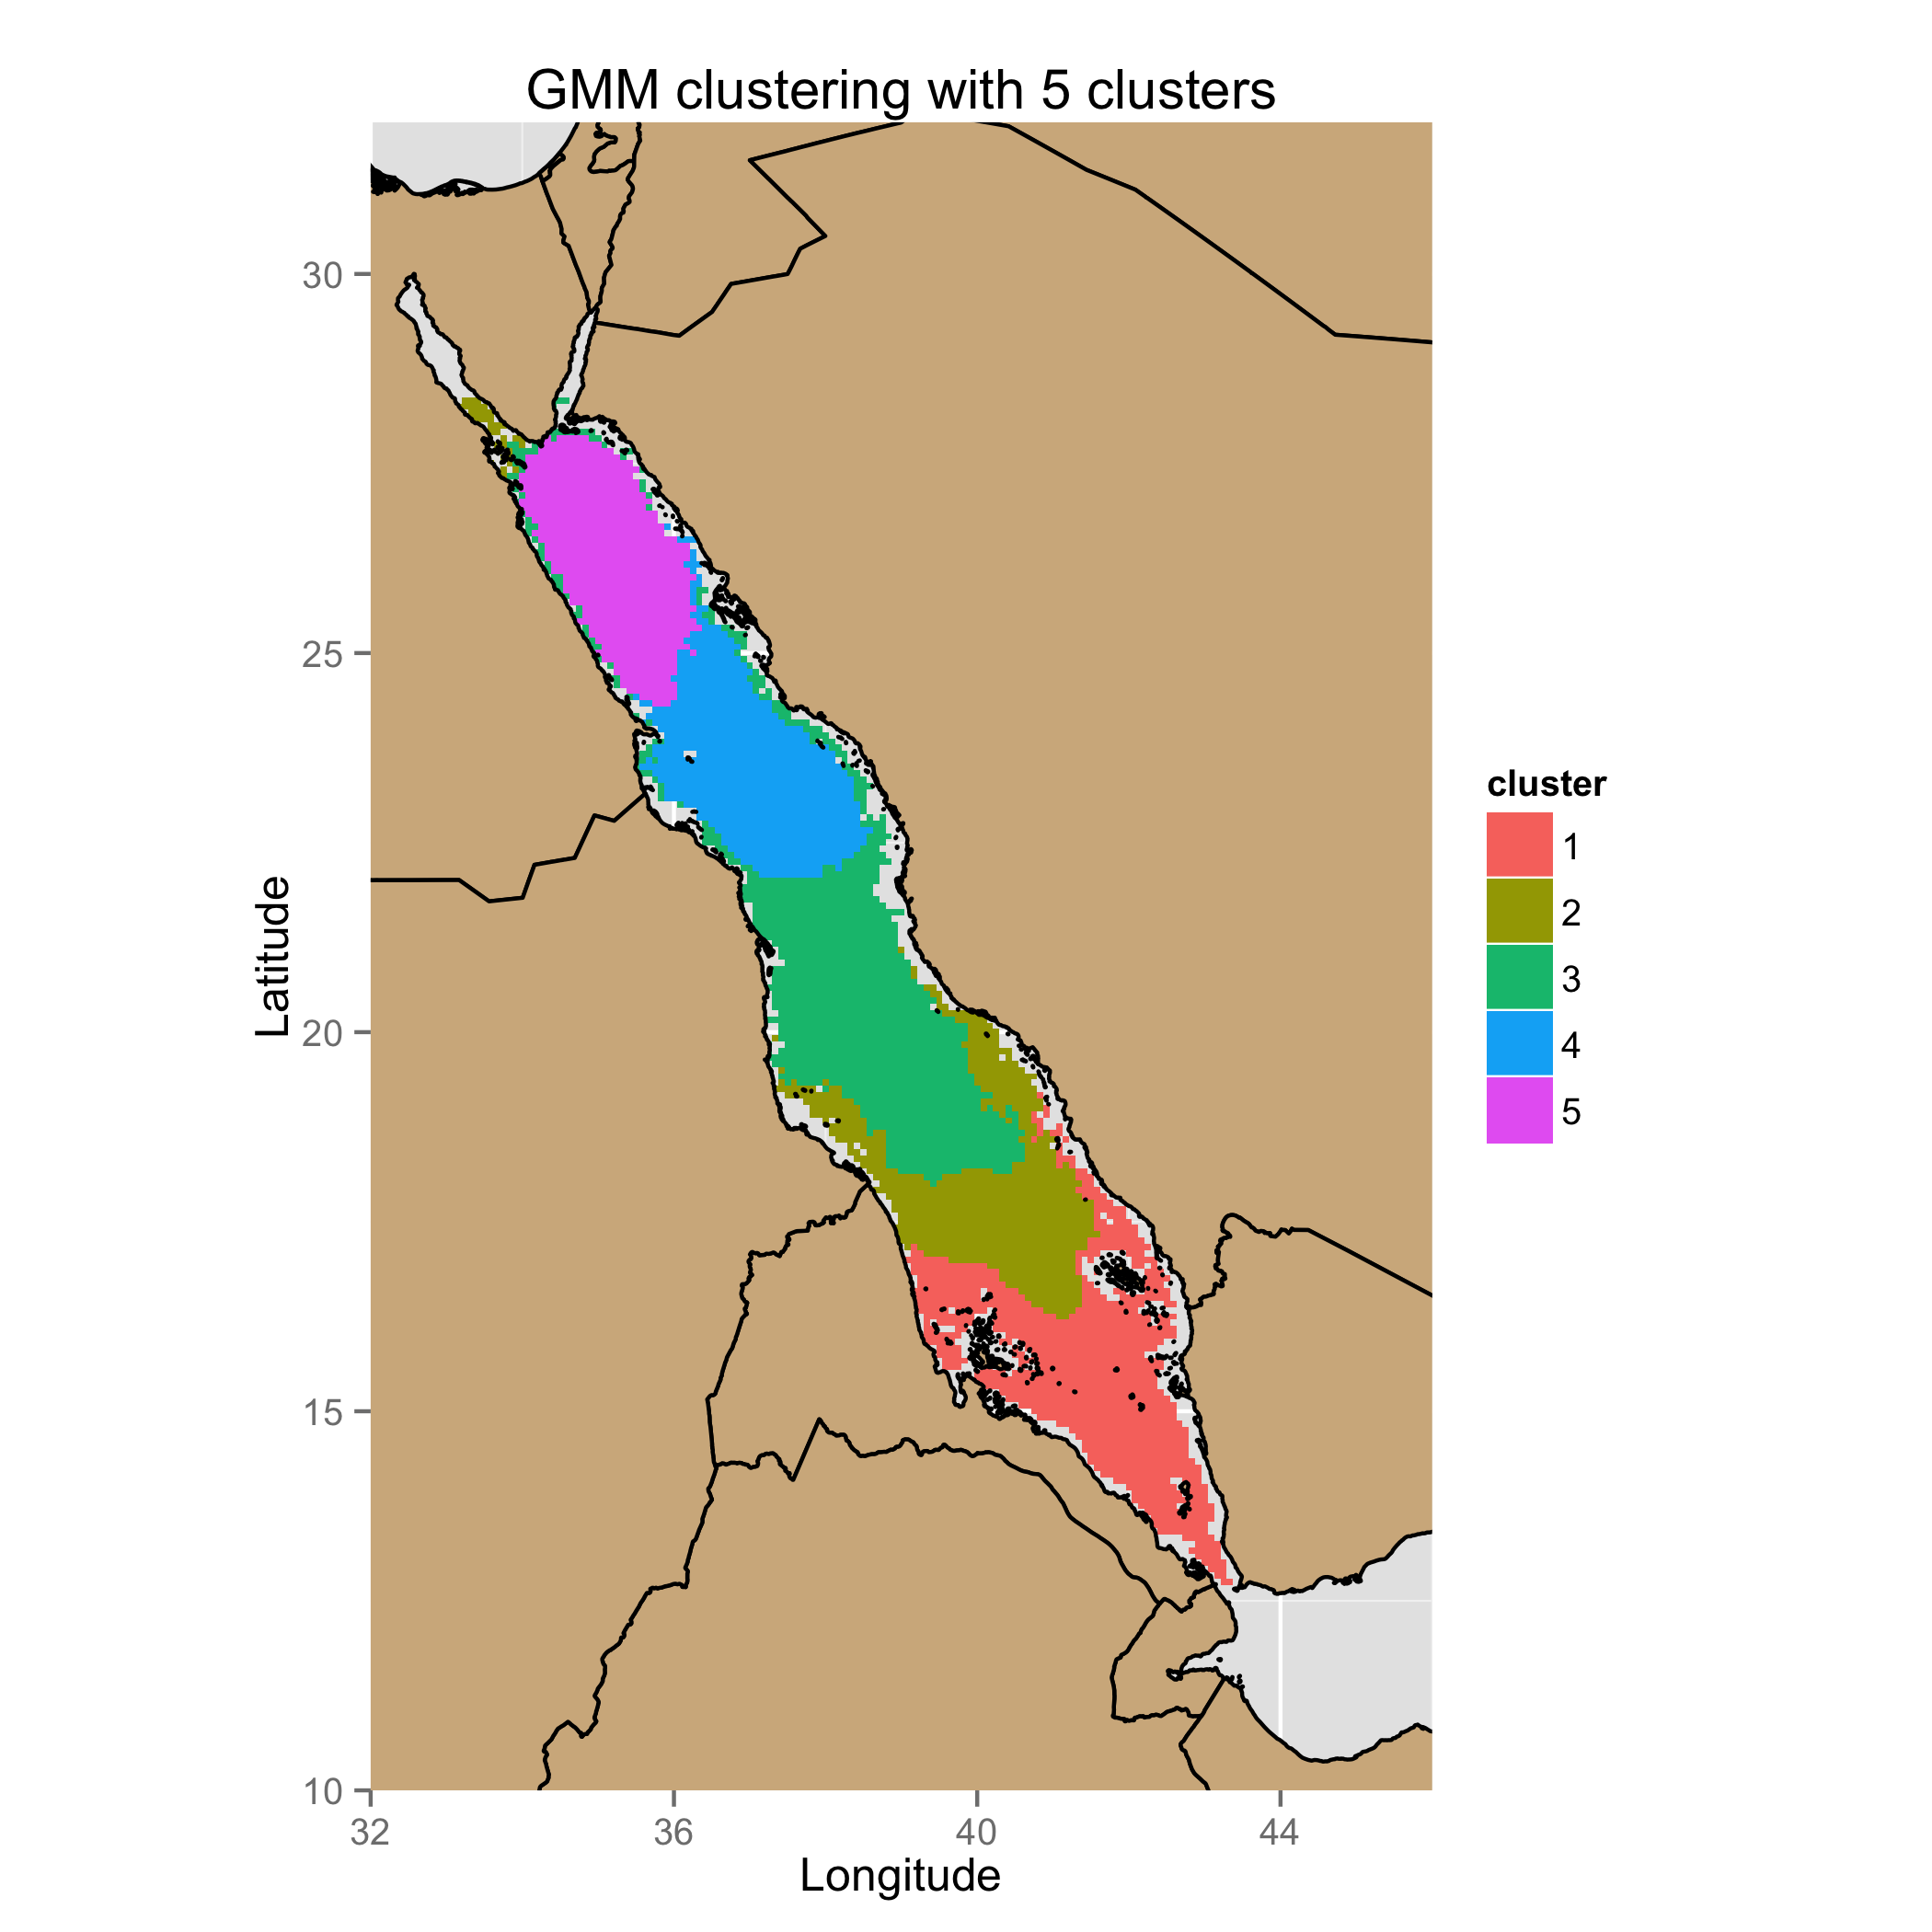
\includegraphics[scale=.15]{figures/clusters_k5.png}
    \caption{Clustering of Red Sea using GMM, with filled monthly SeaWiFS
             chlorophyll data.}
    \label{cluster}
\end{figure}

In Chapter 2, I plan to use the dataset constructed in Chapter 1.  By using CCI
chlorophyll data instead of SeaWiFS, the need for data filling is minimized.
This is desirable, as data filling can introduce biases. It will also be
possible to use additional variables. For example, we can expect the
temperature and the bathymetry to have a large impact on the Red Sea
phytoplankton biology. Sea level anomaly can be useful in that it indicates the
presence of mesoscale eddies. Finally, alternative clustering algorithms will
be tested.

\section{Global Geostatistical Model}

The research described in Chapter 3 of the thesis has mostly been
done and, is the object of an article currently in review. The current version
of the manuscript can be found in appendice. We include the abstract below:

\begin{quotation}
A statistical model is proposed to filter satellite-derived chlorophyll
concentration from the Red Sea, and to predict future chlorophyll
concentrations. The seasonal trend is first estimated after filling missing
chlorophyll data using an Empirical Orthogonal Function (EOF)-based algorithm
(Data Interpolation EOF). The anomalies are then modeled as a stationary
Gaussian process. A method proposed by \citet{Gneiting2002} is used to
construct positive-definite space-time covariance models for this process.
After choosing an appropriate statistical model and identifying its parameters,
Kriging is applied in the space-time domain to make a one step-ahead prediction
of the anomalies. The latter serves as the prediction model of a reduced-order
Kalman filter, which is applied to assimilate and predict future observations
of chlorophyll concentrations. The proposed method decreases the root mean
square (RMS) prediction error by about 11\% compared with the seasonal
prediction.
\end{quotation}

\section{Regional 1D Ecological Models}

The 1D regional ecological models used for this thesis have been configured and
are operational. Three models will be used: for the northern, central and
southern Red Sea. The extreme south of the Red Sea is not modeled, as its
dynamics is poorly understand and no in situ data are available to validate the
satellite products. The ecology is modeled with ERSEM, and the hydrodynamics
is modeled with the MITgcm.

The results of the MITgcm are those from \citet{Yao2014, Yao2014b}, in which a
simulation of the Red Sea and part of the Gulf of Aden circulation was run over
50 years. The NCEP data were used for atmospheric forcing, and the ocean ECCO
data for the open boundary conditions in the Gulf of Aden. The output of the 50
years run are used for the temperature and vertical circulation at the modeled
points.

ERSEM simulates the complete water column with the pelagic and benthic
ecosystems, as well a their coupling. The equations model the flow of carbon,
nitrogen, phosphorus and silicon in the ecosystem. Living organisms are modeled
in terms of population processes (growth and mortality) and physiological
processes (ingestion, respiration, excretion, and egestion). The biota is
divided into functional groups according to their trophic levels: producers
(phytoplankton), consumers (zooplankton) and decomposers (bacteria), and
further subdivided according to their sizes \citep{Baretta1995}.

The ecological models are initialized with the results of a 3D ecological
simulation of the Red Sea \citep{Triantafyllou2014}. The nutrient
concentrations are initialized using values from the World Ocean Atlas 2005
(WOA 2005).

\section{Data Assimilation into the 1D Ecological Models}

The assimilation scheme for the ecological models has been implemented and is
operational. The chosen scheme is a hybrid-SEIK, with the hybrid approach
implemented as described in \citet{Hamill2000}.  The scheme is called hybrid as
it combines the flow-dependent background estimates from the ensemble of an
EnKF with as static background, taken for example from a three-dimensional
variational 3DVAR system. The idea behind it is to complete the rank-deficient
EnKF background by another background that has been designed to capture the
climatological variability of the system.  In our hybrid implementation, the
covariance is a linear combination of the 3DVAR covariance and the
time-evolving SEIK covariance matrix. Figure \ref{assim} shows the assimilation
scheme improves the fit of the model to the chlorophyll data.

The problem of optimal filtering can be solved exactly by the Kalman Filter for
linear systems. For nonlinear models, one can use the Extended Kalman (EK)
filter, in which the model is linearized by computing the error covariance
function.  However, when the state is large, as is often the case for
oceanographic applications, the EK is intractable. In that case, SEEK can be
used, where the error covariance function is projected into a smaller subspace.
This subspace evolves to ensure that most of the error is represented and
filtered out. SEIK can be viewed as an ensemble variant of the SEEK, where the
error covariance function is represented exactly by an ensemble of states. This
avoids the computation of model gradients, and allows the assimilation scheme
to perform better when this model is strongly non-linear. SEIK has been shown
to be efficient for large-scale 3D ecosystem data assimilation
\citep{Triantafyllou2003}.

\begin{figure}
    \centering
    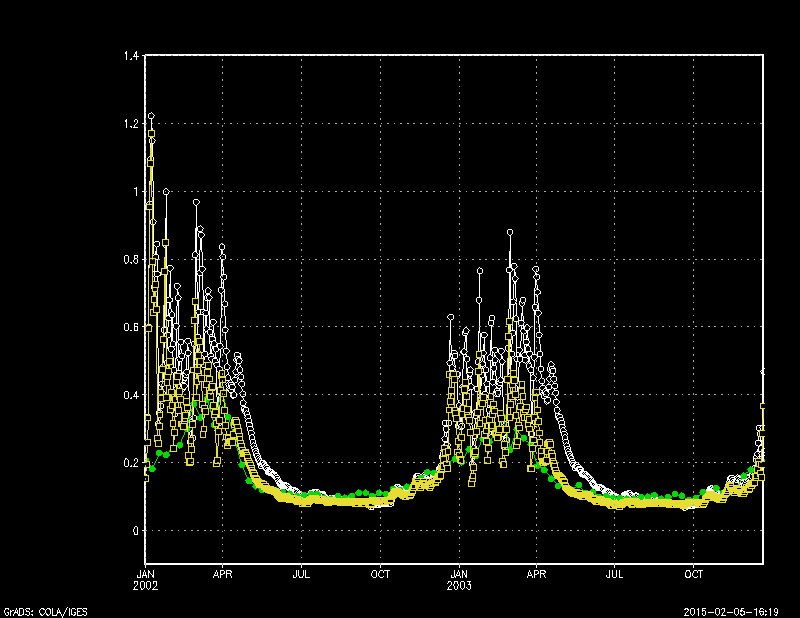
\includegraphics[scale=.45]{figures/chl_factor.png}
    \caption{Surface chlorophyll in the northern Red Sea from CCI data (green),
             from a free run of the 1D ecological model (white), with data
             assimilation (yellow)}
    \label{assim}
\end{figure}


The Expectation-Maximization scheme to estimate the filter parameters has also
been derived. It is similar to that proposed by \citet{Tandeo2014}, 
except that the model is nonlinear. The scheme will be used to improve
the estimates of the observation and model covariance errors.
